% Set the author and title of the compiled pdf
\hypersetup{
	pdftitle = {\Title},
	pdfauthor = {\Author}
}

\section{Introduction}

We want computers to be able to interact with us, just like we interact with
them. This involves having them understand written text and voiced speech, as
well as being able to synthesise speech and text themselves. This includes
things like translation text and searching for key words in text.

A computer or a suite of programs that can do all of this is the goal for
Natural Language Systems. The catch is, that language is hard and complicated,
and to make computers do the things we want them to, we need to know how3
language works, and express this as an executable program.

Language is the representation of ideas, and the linkage of different ideas
together in such a way as to create new ideas. In order to understand any one
sentence (a sentence usually corresponds to one idea, event or action), we have
to understand what each symbol in the language means in isolation, and
understand how they're connected, and what the connections to do change the
meaning of the ideas.

Many factors affect the meaning of a sentence, but the connection between words
is always hierarchical, and we can represent sentences as trees:

\begin{figure}[ht]
  \centering
  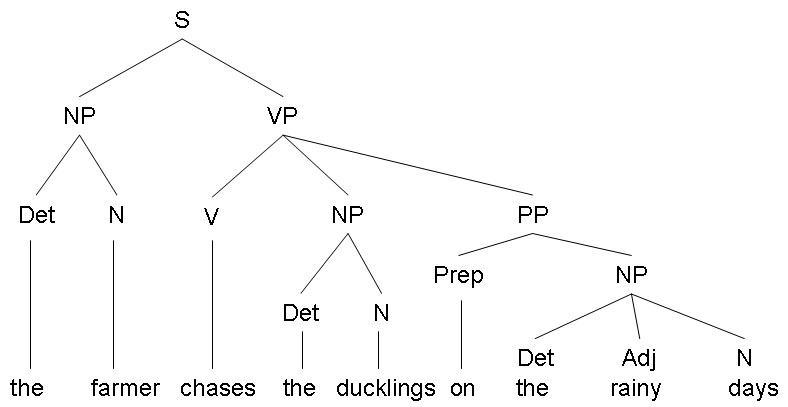
\includegraphics[width=0.55\textwidth]{images/phase-structure-tree}
  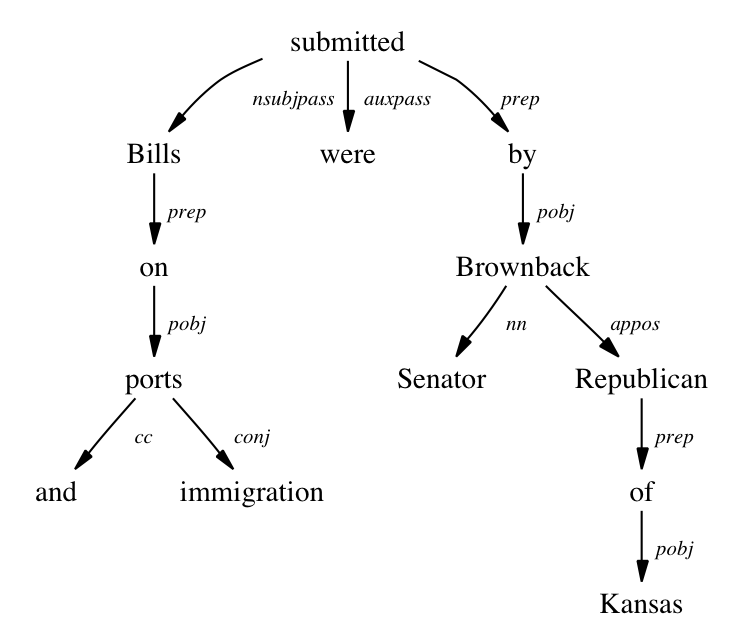
\includegraphics[width=0.35\textwidth]{images/dependency-tree}
  \caption{The left image is a phase structure tree, and the right image is a
  dependency tree.}
  \label{fig:trees}
\end{figure}

A parse tree is all well and good, but to a computer, this is only slightly more
useful than the original text. Though we have extracted some information out of
the text, we still just have a hierarchy of words, but we want a hierarchy of
ideas.

Having ideas instead of words allows us to infer more than what the text
literally says:

\begin{itemize}
  \item I'm fixing my motorbike $\rightarrow$ This person possesses a
  motorbike, and it is currently broken.
  \item The cake smells good $\rightarrow$ There is cake somewhere. Somebody is
  close enough to smell it.
\end{itemize}

But how can we do that?

\section{Structural analysis}

It is possibly to try and find out the meaning of a word simply by looking at
what letters it is made up of. One way to do this is to split a word into
\textbf{morphemes}, which are the most basic meaning-carrying components of a
word, and try to associate a meaning with each. For example \textit{undone}
could be split into \textit{un} and \textit{done}, and meaning associated with
each.

\subsection{Tries}

\marginpar{Tries are very handy datastructures for technical interviews, you
should read up on them an implement one!}

In order to examine the syntactic and semantic properties of the words, we need to represent them in the computer. A common way to do this is with a \textit{trie}:

\begin{wrapfigure}{r}{0.25\textwidth}
  \begin{center}
    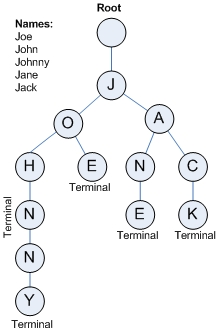
\includegraphics[width=0.24\textwidth,keepaspectratio]{images/trie}
  \end{center}
  \caption{A trie storing some names.}
\end{wrapfigure}

Tries are very memory efficient, since they if multiple words share the same
prefix, then the prefix is only stored once in memory. Tries have a lookup time
of $O(m)$, where $m$ is the length of the word, which is quite good, and is
better than a hash table in terms of speed in some cases. If you're stupid
enough to represent your dictionary as a list of words, then you can do a binary
search if its ordered (worst case $O(log(n) * m)$ comparisons (the $m$ comes
from having to possibly compare each character in the word)), or a linear search
if it isn't ordered ($O(m*n)$ in the worst case!).

\subsection{Spelling rules}

We want to understand why combining \textit{big} and \textit{est} produces
\textit{biggest} with an extra \textit{g}. Why isn't it \textit{bigest}? The
reason why we want to understand this, is so we can go from a word that we're
processing in text, and pick it apart into its components so we can better
understand it.

That is to say, we're going from \textit{biggest} to \textit{big} +
\textit{est}.

The format of the rules we're using in the course is as follows:

\marginpar{You can use \texttt{cX} and \texttt{vX} where \texttt{X} is an
integer, and \texttt{c/v} denotes a consonant or vowel inside the context
brackets.}

\begin{verbatim}
  [from] ==> [to]: [prevContext] _ [nextContext];
\end{verbatim}

For example, if we had a rule like:

\begin{verbatim}
  [g] ==> []: [g] _ [e,s,t];
\end{verbatim}

It would turn \textit{biggest} into \textit{big} + \textit{est}.

\subsection{Categorical descriptions}

Even if we find the meaning of every word by splitting it info morphemes, we
just end up with a collection of words that we know the construction of, but
we're still no closer to understanding a sentence.

In order to find the relationships between words in a sentence, we should use
the approach in Figure~\ref{fig:trees}, and try to fit the words into some tree
structure.

One way of doing this, is to specify lots of different forms that a sentence can
take. For example `noun verb noun' might describe a sentence such as `Todd
writes notes'. Providing that we have some \textit{prototype} for a sentence
that fits the words that we've been given, we can ascertain that we can in fact
make a sentence out of these words.

There is a better approach though. Each word in a sentence changes its meaning
in some way, and we can put words into buckets according to how the meaning of
the sentence is changed; for example, a verb specifies what kind of event is
happening. Having a verb on its own doesn't do us much good; we will know that
\textit{something} is happening, but not where, why, what, when etc. Verbs need
other parts of sentence around them to make them work.

We can treat each word as part of a jigsaw, specifying what other words or
phrases it needs in order to have meaning, and then fit the pieces together
according to some schema.

We need to specify a schema with which we can specify what different words require:

\begin{verbatim}
  <word> = <rules>
\end{verbatim}

The rules are their own language, which has a few rules. Brackets are
treated as they usually are in maths, and the only other special characters are
forward and backward slashes. These indicate whether a word or phrase should be
before or after the word.

\begin{verbatim}
  writes = (s\np)/np
\end{verbatim}

This indicates that the word `writes' needs a noun phrase (\texttt{np}) to its
right and then a noun phrase to its left to make a sentence (\texttt{s}).

With the right set of rules for each word, we can now parse sentences:

\begin{verbatim}
  writes = (s\np)/np
  Todd = np
  notes = np
\end{verbatim}

\begin{center}
  % Tabular centering hack
  \begin{tabular}{c}
    \begin{lstlisting}
      Todd        writes        notes
       np       (s\np)/np        np
                ---------------------
                        s\np
      -----------------------
                s
    \end{lstlisting}
  \end{tabular}
\end{center}

Here, the words `Todd' and `notes' are \textit{saturated} since they don't
require anything else to make them into complete `items'. `writes' is
unsaturated, since it needs other stuff to make it into a complete item. Word
rules of these kind are called \textbf{Categorical Descriptions}.

\subsection{Morphology}

Now we've figured out how to decompose a word into morphemes using spelling
rules, and we can fit these words into a sentence. However, we also want to know the precise meaning for each word (this helps when arranging them in a sentence too). We can do this by looking at each morpheme.

There are two types of morphology that we're going to look at:

\begin{description}
  \item \textbf{Inflectional morphology}\\
    This is when the stem of the word is incomplete, and other morphemes 
    provide more information to specify exactly what we mean:

    \begin{itemize}
      \item `sing' + `ing' = verb + present participle
      \item `work' + `ed' = verb + past participle
      \item `work' + `' = noun + singular
    \end{itemize}

  \item \textbf{Derivational morphology}\\
    This is where the meaning of the stem is significantly changed by other 
    morphemes. For example, `smelly' could be combined with `er' to give 
    `smellier', or `est' to give `smelliest'. Obviously we need spelling rules 
    to do this correctly!
\end{description}

We need a way to specify what words can have what suffixes/affixes. For example,
`conscript' can be combined with `tion' to give `conscription', but not `ly' to
give `conscriptly'.

Furthermore, there are spelling rules concerned with adding bits onto words; as
we saw before, `smelly' becomes `smellier', not `smellyer'. We will come across
this later though.

It turns out that composing morphemes is similar to composing words. We can use the same notation:

\begin{verbatim}
  'conscript' = noun>agr
  'conscript' = verb>tns
  'tion' = (noun>agr)<(verb>tns)
  'ing' = tns
  'ed' = tns
  's' = agr
  '' = agr
\end{verbatim}

These descriptions allow you to construct the following words:

\begin{mymulticols}
  \begin{itemize}
    \item conscript (noun)
    \item conscripts (noun)
    \item conscription (noun)
    \item conscriptions (noun)
    \item conscripting (verb)
    \item conscripted (verb)
  \end{itemize}
\end{mymulticols}

However, the rules are not perfect, and will also allow you to make:

\begin{mymulticols}
  \begin{itemize}
    \item conscriptingtion (noun)
    \item conscriptedtion (noun)
    \item conscriptingtions (noun)
    \item conscriptedtions (noun)
  \end{itemize}
\end{mymulticols}

We can also make rules cancel out. If we have a rule that is `verb$>$tns' and
another that is `tns$>$agr' then we can make a `verb$>$agr' from them.

To see a worked example of these rules, and how they're applied, look on slides
$64-110$ in the
\href{http://studentnet.cs.manchester.ac.uk/ugt/2015/COMP34411/COMP34411.pdf}
{course notes}.

One thing that is important to note, is that we can process words from left to
right, and don't have to back-track. This means that processing is in linear
time, which is fantastic (though we need a big dictionary of words, which is
rather less fantastic).

\subsection{Unknown words}

Now we can read in a sentence, parse each word and extract the relations between
the words to produce a meaningful parse tree, great! But\dots what if we
don't have a word in the input sentence in our dictionary? We won't be able to
fit it into our parse tree since it won't have any meaning to us. Looking at the
morphemes doesn't tell us too much; having `ing' at the end means that a word is
probably a verb and is in the present tense, but doesn't tell us what's actually
going on.

There are two different classes of classes of words \textit{open} and
\textit{closed}. Open classes are verbs, adjectives, nouns etc where there are
lots of them and you can easily add more (new nouns are created all the time).
Closed classes are things like prepositions (`in', `on'), and auxiliaries (`be',
`have', `would') where you rarely if ever get new words being added.

So, if we cannot recognise a word using the morphological rules we used before,
then we should \textbf{back off} to using a more robust but less accurate
strategy. Lets define exactly what robust and accurate mean:

\begin{description}
  \item \textbf{Robust}\\
    This is when a system always gives an answer, even if the answer might be 
    wrong. It's sometimes a good idea have a robust system, since then you can 
    always take \textit{some} action.
  \item \textbf{Accurate}\\
    An accurate system always gets the answer `right' when asked a question.
\end{description}

A common strategy in Natural Language Processing is to use a system that is
highly accurate but less robust, but fall back on a less accurate but more
robust system when the first doesn't give an answer.

So, we need to build a robust word recogniser for unknown words. To do this, we
need to know what word it is, and what part of speech tag it has (noun, verb
etc).

\subsubsection{Stemming}

If you were to come across the word `blodge', you probably wouldn't know what it
means (althought there are, as always a number of definitions in the
\href{http://www.urbandictionary.com/define.php?term=blodge}{Urban Dictionary}).
If a word like `blodge' were to appear in the middle of a sentence, you could
probably still extract some information from it:

\begin{itemize}
  \item I went to blodge $\rightarrow$ Blodge is a place.
  \item I went to blodged it $\rightarrow$ Blodging is a thing you can do.
    The blodging happened in the past.
  \item The car was blodge $\rightarrow$ You can describe something as having 
    the property/quality `blodge'.
\end{itemize}

The \textbf{Porter Stemmer} is a set of rules that tell you what bits of a word
you can remove to get the stem of the word that is common to all forms of the
word. If we run the porter stemmer on `blodge', `blodging' and `blodged', then
we get the stem as `blodg'. Now we can at least identify all instances of
`blodg*' as the same word.

\subsubsection{Part of speech tagging}

When we look up a word in a dictionary, we get something like this:

\begin{figure}[H]
  \centering
  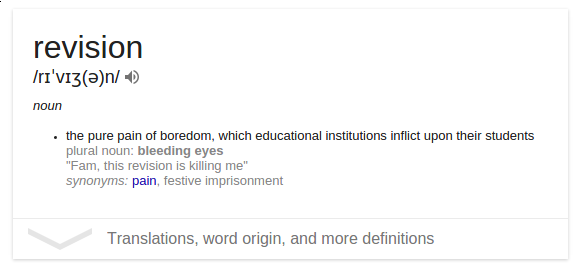
\includegraphics[width=0.75\textwidth]{images/revision-definition}
  \caption{A dictionary definition of the word `revision'.}
  \label{fig:revision-definition}
\end{figure}

Not only does a dictionary give us the definition of a word, but it also give us
its part of speech tag. In the case of Figure~\ref{fig:revision-definition} it
is a noun. We need the POS tag in order to work out how words are related to
each other, so we can put them in their proper place in a parse tree.

There are a number of ways to do part of speech tagging (this is what I'm doing
for my third year project, and it's a rabbit hole that you don't want to go down
if you're trying to revise for exams). Here are the ones you need to know for
this course:

\begin{description}

  \marginpar{One thing to be aware of with using corpuses, is that they are 
  often ordered. If you use the first $N$ million words for training and the 
  next $M$ million for testing, then you could end up with disasterous results, 
  because different areas of the corpus will be about different genres, and 
  will contain different words.}

  \item \textbf{Dictionary look up}\\
  The easiest way to do POS tagging (but also the worst), is to get a big
  massive dictionary, and find the part of speech tag for each word. Then, when
  you need to tag a word, then you just look it up in your big list.

  However, you need lots and lots and lots of words to do this, and getting the
  tags for all of the words is a big task. Furthermore, if we're trying to
  handle unknown words, then by definition, we've not seen them before and they
  won't be in our dictionary.

  Obviously, the bigger your list of words, the fewer words you'll need to
  handle. The British National Corpus has 100 million words in, which is in the
  right ballpark, but it is poorly tagged (the error rate is above 1\% in
  parts). Other corpuses are available, but are either smaller, or you have to
  pay for them. In order to use the BNC (or any corpus) as a dictionary, you
  count how many times each word is tagged with each part of speech tag, and
  then assign the most common tag.

  There are two main advantages to this method; first of all, it's really
  simple, and computationally easy. Using a sensible hash table, lookup is
  $O(1)$ and training is $O(n)$. It's so fast that the bottleneck is usually the
  IO operations of reading (and decoding) the corpus. The second advantage, is
  that you get alternative tags for words. A word might be in the corpus 50
  times as a verb, but 20 times as a noun, and you can use this information in
  your processing.

  As a \textbf{backoff} technique, you can also keep track of the POS
  probabilities for the last $n$ letters of the word, so if the word isn't in
  your dictionary, you can use the last $n$ letters of it to determine what tag
  to assign.

  %TODO: Sefine precision and recall somewhere

  \item \textbf{Transition probabilities and HMM's}\\

  HMM's use probabilities and context to determine what tag a word should get.
  To train a HMM, we collect statistics on what part of speech tags
  \textit{follow and precede} other ones. For example, the probability of a noun
  being followed by another noun might be quite high, because of names (e.g.
  Todd Davies), and adjectives usually lead onto nouns, or other adjectives
  (e.g. hungry bored Todd).

  These are called \textbf{bigram} probabilities (because you have information
  about following and preceding tags). A HMM based POS tagger works as follows:

  \begin{itemize}
    \item For each word, use a corpus to calculate how likely it is to belong 
    to each class (just like we did for the dictionary look up approach). These 
    are the emission probabilities.
    \item For each tag that we have found that might correspond to a specific 
    word, look at the tag we assigned to the previous (and possibly next) word(
    s) and use the transition probabilities to choose the most likely tag.
  \end{itemize}

  We want to find the most likely sequence of tags for the whole sentence, which
  is why the hidden markov model works well. However, training can be slow and
  its hard to make use of the backward transition probabilities.

  \marginpar{I think this is more important for the POS tagging part of the
  course than HMM's are.}

  Alternately, you can use no HMM at all, by using a function to evaluate the
  best next tag:

  \[
    \begin{split}
    F(&dict(Word, tag_i),\\
      &\sum_k(P(tag(prevWord) = tag_k) \times P(tag_k \rightarrow tag_i)),\\
      &\sum_k(dict(nextWord, tag_k) \times P(tag_i \leftarrow tag_k)))
    \end{split}
  \]

  You can define $F$ to be anything, but in the course notes:

  \[
    F(dictProbability, forward, backward) = \sqrt{dictProbability} \times 
      (forward + backward)
  \]

\end{description}